%%% Hlavní soubor. Zde se definují základní parametry a odkazuje se na ostatní části. %%%

%% Verze pro jednostranný tisk:
% Okraje: levý 40mm, pravý 25mm, horní a dolní 25mm
% (ale pozor, LaTeX si sám přidává 1in)
\documentclass[12pt,a4paper]{report}
\setlength\textwidth{145mm}
\setlength\textheight{247mm}
\setlength\oddsidemargin{15mm}
\setlength\evensidemargin{15mm}
\setlength\topmargin{0mm}
\setlength\headsep{0mm}
\setlength\headheight{0mm}
% \openright zařídí, aby následující text začínal na pravé straně knihy
\let\openright=\clearpage

%% Pokud tiskneme oboustranně:
% \documentclass[12pt,a4paper,twoside,openright]{report}
% \setlength\textwidth{145mm}
% \setlength\textheight{247mm}
% \setlength\oddsidemargin{15mm}
% \setlength\evensidemargin{0mm}
% \setlength\topmargin{0mm}
% \setlength\headsep{0mm}
% \setlength\headheight{0mm}
% \let\openright=\cleardoublepage

%% Použité kódování znaků: obvykle latin2, cp1250 nebo utf8:
\usepackage[utf8]{inputenc}

%% Ostatní balíčky
\usepackage{graphicx}
\usepackage{amsthm}

%% My packages:
\usepackage{algorithm}
\usepackage{algpseudocode}
\usepackage{commath}
\usepackage{float}
\floatstyle{ruled} \newfloat{pseudocode}{thp}{lop} \floatname{pseudocode}{Pseudocode}
\usepackage{color}
\definecolor{lightgray}{rgb}{0.95, 0.95, 0.95}
\definecolor{darkgray}{rgb}{0.4, 0.4, 0.4}
\definecolor{purple}{rgb}{0.65, 0.12, 0.82}
%\definecolor{editorGray}{rgb}{0.95, 0.95, 0.95}
\definecolor{editorGray}{rgb}{1, 1, 1}
\definecolor{editorOcher}{rgb}{1, 0.5, 0} % #FF7F00 -> rgb(239, 169, 0)
\definecolor{editorGreen}{rgb}{0, 0.5, 0} % #007C00 -> rgb(0, 124, 0)
\usepackage{upquote}
\usepackage{listings}
% CSS
\lstdefinelanguage{CSS}{
  keywords={color,background-image:,margin,padding,font,weight,display,position,top,left,right,bottom,list,style,border,size,white,space,min,width, transition:, transform:, transition-property, transition-duration, transition-timing-function},	
  sensitive=true,
  morecomment=[l]{//},
  morecomment=[s]{/*}{*/},
  morestring=[b]',
  morestring=[b]",
  alsoletter={:},
  alsodigit={-}
}

% JavaScript
\lstdefinelanguage{JavaScript}{
  morekeywords={typeof, new, true, false, catch, function, return, null, catch, switch, var, if, in, while, do, else, case, break},
  morecomment=[s]{/*}{*/},
  morecomment=[l]//,
  morestring=[b]",
  morestring=[b]'
}

\lstdefinelanguage{HTML5}{
  language=html,
  sensitive=true,	
  alsoletter={<>=-},	
  morecomment=[s]{<!-}{-->},
  tag=[s],
  otherkeywords={
  % General
  >,
  % Standard tags
	<!DOCTYPE,
  </html, <html, <head, <title, </title, <style, </style, <link, </head, <meta, />,
	% body
	</body, <body,
	% Divs
	</div, <div, </div>, 
	% Paragraphs
	</p, <p, </p>,
	% scripts
	</script, <script,
  % More tags...
  <canvas, /canvas>, <svg, <rect, <animateTransform, </rect>, </svg>, <video, <source, <iframe, </iframe>, </video>, <image, </image>
  },
  ndkeywords={
  % General
  =,
  % HTML attributes
  charset=, src=, id=, width=, height=, style=, type=, rel=, href=,
  % SVG attributes
  fill=, attributeName=, begin=, dur=, from=, to=, poster=, controls=, x=, y=, repeatCount=, xlink:href=,
  % CSS properties
  margin:, padding:, background-image:, border:, top:, left:, position:, width:, height:,
	% CSS3 properties
  transform:, -moz-transform:, -webkit-transform:,
  animation:, -webkit-animation:,
  transition:,  transition-duration:, transition-property:, transition-timing-function:,
  }
}

\lstset{%
  % General design
  backgroundcolor=\color{editorGray},
  basicstyle={\small\ttfamily},   
  frame=l,
  % line-numbers
  xleftmargin={0.75cm},
  numbers=left,
  stepnumber=1,
  firstnumber=1,
  numberfirstline=true,	
  % Code design
  identifierstyle=\color{black},
  keywordstyle=\color{blue}\bfseries,
  ndkeywordstyle=\color{editorGreen}\bfseries,
  stringstyle=\color{editorOcher}\ttfamily,
  commentstyle=\color{darkgray}\ttfamily,
  % Code
  language=HTML5,
  alsolanguage=JavaScript,
  alsodigit={.:;},	
  tabsize=2,
  showtabs=false,
  showspaces=false,
  showstringspaces=false,
  extendedchars=true,
  breaklines=true,
  % German umlauts
  literate=%
  {Ö}{{\"O}}1
  {Ä}{{\"A}}1
  {Ü}{{\"U}}1
  {ß}{{\ss}}1
  {ü}{{\"u}}1
  {ä}{{\"a}}1
  {ö}{{\"o}}1
}
\usepackage{caption}
\captionsetup[lstlisting]{position=bottom}

%%% Drobné úpravy stylu

% Tato makra přesvědčují mírně ošklivým trikem LaTeX, aby hlavičky kapitol
% sázel příčetněji a nevynechával nad nimi spoustu místa. Směle ignorujte.
\makeatletter
\def\@makechapterhead#1{
  {\parindent \z@ \raggedright \normalfont
   \Huge\bfseries \thechapter. #1
   \par\nobreak
   \vskip 20\p@
}}
\def\@makeschapterhead#1{
  {\parindent \z@ \raggedright \normalfont
   \Huge\bfseries #1
   \par\nobreak
   \vskip 20\p@
}}
\makeatother

% Toto makro definuje kapitolu, která není očíslovaná, ale je uvedena v obsahu.
\def\chapwithtoc#1{
\chapter*{#1}
\addcontentsline{toc}{chapter}{#1}
}

%\usepackage{color}
\definecolor{lightgray}{rgb}{0.95, 0.95, 0.95}
\definecolor{darkgray}{rgb}{0.4, 0.4, 0.4}
\definecolor{purple}{rgb}{0.65, 0.12, 0.82}
%\definecolor{editorGray}{rgb}{0.95, 0.95, 0.95}
\definecolor{editorGray}{rgb}{1, 1, 1}
\definecolor{editorOcher}{rgb}{1, 0.5, 0} % #FF7F00 -> rgb(239, 169, 0)
\definecolor{editorGreen}{rgb}{0, 0.5, 0} % #007C00 -> rgb(0, 124, 0)
\usepackage{upquote}
\usepackage{listings}
% CSS
\lstdefinelanguage{CSS}{
  keywords={color,background-image:,margin,padding,font,weight,display,position,top,left,right,bottom,list,style,border,size,white,space,min,width, transition:, transform:, transition-property, transition-duration, transition-timing-function},	
  sensitive=true,
  morecomment=[l]{//},
  morecomment=[s]{/*}{*/},
  morestring=[b]',
  morestring=[b]",
  alsoletter={:},
  alsodigit={-}
}

% JavaScript
\lstdefinelanguage{JavaScript}{
  morekeywords={typeof, new, true, false, catch, function, return, null, catch, switch, var, if, in, while, do, else, case, break},
  morecomment=[s]{/*}{*/},
  morecomment=[l]//,
  morestring=[b]",
  morestring=[b]'
}

\lstdefinelanguage{HTML5}{
  language=html,
  sensitive=true,	
  alsoletter={<>=-},	
  morecomment=[s]{<!-}{-->},
  tag=[s],
  otherkeywords={
  % General
  >,
  % Standard tags
	<!DOCTYPE,
  </html, <html, <head, <title, </title, <style, </style, <link, </head, <meta, />,
	% body
	</body, <body,
	% Divs
	</div, <div, </div>, 
	% Paragraphs
	</p, <p, </p>,
	% scripts
	</script, <script,
  % More tags...
  <canvas, /canvas>, <svg, <rect, <animateTransform, </rect>, </svg>, <video, <source, <iframe, </iframe>, </video>, <image, </image>
  },
  ndkeywords={
  % General
  =,
  % HTML attributes
  charset=, src=, id=, width=, height=, style=, type=, rel=, href=,
  % SVG attributes
  fill=, attributeName=, begin=, dur=, from=, to=, poster=, controls=, x=, y=, repeatCount=, xlink:href=,
  % CSS properties
  margin:, padding:, background-image:, border:, top:, left:, position:, width:, height:,
	% CSS3 properties
  transform:, -moz-transform:, -webkit-transform:,
  animation:, -webkit-animation:,
  transition:,  transition-duration:, transition-property:, transition-timing-function:,
  }
}

\lstset{%
  % General design
  backgroundcolor=\color{editorGray},
  basicstyle={\small\ttfamily},   
  frame=l,
  % line-numbers
  xleftmargin={0.75cm},
  numbers=left,
  stepnumber=1,
  firstnumber=1,
  numberfirstline=true,	
  % Code design
  identifierstyle=\color{black},
  keywordstyle=\color{blue}\bfseries,
  ndkeywordstyle=\color{editorGreen}\bfseries,
  stringstyle=\color{editorOcher}\ttfamily,
  commentstyle=\color{darkgray}\ttfamily,
  % Code
  language=HTML5,
  alsolanguage=JavaScript,
  alsodigit={.:;},	
  tabsize=2,
  showtabs=false,
  showspaces=false,
  showstringspaces=false,
  extendedchars=true,
  breaklines=true,
  % German umlauts
  literate=%
  {Ö}{{\"O}}1
  {Ä}{{\"A}}1
  {Ü}{{\"U}}1
  {ß}{{\ss}}1
  {ü}{{\"u}}1
  {ä}{{\"a}}1
  {ö}{{\"o}}1
}

\usepackage{footnote}
\usepackage{array}
\newcolumntype{L}[1]{>{\raggedright}m{#1}}
\newcolumntype{C}[1]{>{\centering}m{#1}}

\newcommand{\footnoteremember}[2]{
\footnote{#2}
\newcounter{#1}
\setcounter{#1}{\value{footnote}}
}
\newcommand{\footnoterecall}[1]{
\footnotemark[\value{#1}]
}


\usepackage[refpage]{nomencl}
\usepackage{etoolbox}
\makeatletter
\patchcmd{\thenomenclature}%
  {\chapter*{\nomname}}%
  {\section*{\nomname}}%
  {}{\message{^^Jthenomenclature patching failed (1)^^J}}
\patchcmd{\thenomenclature}%
  {\if@intoc\addcontentsline{toc}{chapter}{\nomname}\fi}%
  {\if@intoc\addcontentsline{toc}{section}{\nomname}\fi}%
  {}{\message{^^Jthenomenclature patching failed (2)^^J}}
\makeatother
\makenomenclature
\renewcommand{\nomname}{} % empty name

\usepackage{pdfpages}



%% Balíček hyperref, kterým jdou vyrábět klikací odkazy v PDF,
%% ale hlavně ho používáme k uložení metadat do PDF (včetně obsahu).
%% POZOR, nezapomeňte vyplnit jméno práce a autora.
\usepackage[ps2pdf,unicode]{hyperref}   % Musí být za všemi ostatními balíčky
%\usepackage[unicode]{hyperref}   % Musí být za všemi ostatními balíčky
\hypersetup{pdftitle=Vector Screencast}
\hypersetup{pdfauthor=Šimon Rozsíval}


\begin{document}

% Trochu volnější nastavení dělení slov, než je default.
\lefthyphenmin=2
\righthyphenmin=2

%%% Titulní strana práce

\pagestyle{empty}
\begin{center}

\large

Charles University in Prague

\medskip

Faculty of Mathematics and Physics

\vfill

{\bf\Large BACHELOR THESIS}

\vfill

\centerline{\mbox{
\includegraphics[width=60mm]{../img/logo.eps}}}

\vfill
\vspace{5mm}

{\LARGE Šimon Rozsíval}

\vspace{15mm}

% Název práce přesně podle zadání
{\LARGE\bfseries Vector Screencast}

\vfill

% Název katedry nebo ústavu, kde byla práce oficiálně zadána
% (dle Organizační struktury MFF UK)
Department of Distributed and Dependable Systems

\vfill

\begin{tabular}{rl}

Supervisor of the bachelor thesis: & Mgr. Martin Děcký \\
\noalign{\vspace{2mm}}
Study programme: & Computer science \\
\noalign{\vspace{2mm}}
Specialization: & Programming and software systems \\
\end{tabular}

\vfill

% Zde doplňte rok
Prague 2015

\end{center}

\newpage

%%% Následuje vevázaný list -- kopie podepsaného "Zadání bakalářské práce".
%%% Toto zadání NENÍ součástí elektronické verze práce, nescanovat.

%%% Na tomto místě mohou být napsána případná poděkování (vedoucímu práce,
%%% konzultantovi, tomu, kdo zapůjčil software, literaturu apod.)

\openright

\noindent
I would like to thank my supervisor, Martin Děcký, for his valuable pieces of advice, and Otakar Jícha from \textit{Khanova Škola}, for the idea of this project and for lending me a graphics tablet for testing.

I would also like to thank my family and friends for supporting me during my studies.



\newpage

%%% Strana s čestným prohlášením k bakalářské práci

\vglue 0pt plus 1fill

\noindent
I declare that I carried out this bachelor thesis independently, and only with the cited
sources, literature and other professional sources.

\medskip\noindent
I understand that my work relates to the rights and obligations under the Act No.
121/2000 Coll., the Copyright Act, as amended, in particular the fact that the Charles
University in Prague has the right to conclude a license agreement on the use of this
work as a school work pursuant to Section 60 paragraph 1 of the Copyright Act.

\vspace{10mm}

\hbox{\hbox to 0.5\hsize{%
In ........ date ............
\hss}\hbox to 0.5\hsize{%
signature of the author
\hss}}

\vspace{20mm}
\newpage

%%% Povinná informační strana bakalářské práce

\vbox to 0.5\vsize{
\setlength\parindent{0mm}
\setlength\parskip{5mm}

Název práce:
Vektorový screencast
% přesně dle zadání

Autor:
Šimon Rozsíval

Katedra:  % Případně Ústav:
Katedra distribuovaných a spolehlivých systémů
% dle Organizační struktury MFF UK

Vedoucí bakalářské práce:
Mgr. Martin Děcký
% dle Organizační struktury MFF UK, případně plný název pracoviště mimo MFF UK

Abstrakt:
Cílem bakalářské práce je vytvořit software pro záznam a přehrávání výukových videí pro potřeby Khanovy školy. Na rozdíl od běžných videí nejsou obrazová data uložena ve formě bitmap, ale jako vektory, což umožní snížit datovou náročnost a vykreslit obraz ostře při libovolně velkém rozlišení obrazovky uživatele. Přehrávač videa i nástroj pro nahrávání běží ve webovém prohlížeči. Součástí práce je také návrh a implementace vhodného formátu pro uchovávání obrazových a zvukových dat a implementace v softwarové architektuře klient/server.
% abstrakt v rozsahu 80-200 slov; nejedná se však o opis zadání bakalářské práce

Klíčová slova:
screencast, vektory, video, on-line

\vss}\nobreak\vbox to 0.49\vsize{
\setlength\parindent{0mm}
\setlength\parskip{5mm}

Title:
Vector Screencast

Author:
Šimon Rozsíval

Department:
Department of Distributed and Dependable Systems
% dle Organizační struktury MFF UK v angličtině

Supervisor:
Mgr. Martin Děcký
% dle Organizační struktury MFF UK, případně plný název pracoviště
% mimo MFF UK v angličtině

Abstract:
The goal of this bachelor thesis is to create a software for recording and playback of educational videos for Khanova škola (Czech clone of Khan Academy). Contrary to common videos the visual data is not stored as a sequence of bitmaps, but as vectors. This allows to reduce the data bandwidth and playback sharp images in any target resolution. The player and also the tool for recording the videos runs in a web browser. The thesis also focuses on designing and implementing a suitable file format for storing the visual and audio data and implementing the software according to the client/server paradigm.
% abstrakt v rozsahu 80-200 slov v angličtině; nejedná se však o překlad
% zadání bakalářské práce

Keywords:
screencast, vector, video, on-line
% 3 až 5 klíčových slov v angličtině

\vss}

\newpage

%%% Strana s automaticky generovaným obsahem bakalářské práce. U matematických
%%% prací je přípustné, aby seznam tabulek a zkratek, existují-li, byl umístěn
%%% na začátku práce, místo na jejím konci.

\openright
\pagestyle{plain}
\setcounter{page}{1}
\tableofcontents

%%% Jednotlivé kapitoly práce jsou pro přehlednost uloženy v samostatných souborech
\chapter*{Introduction}
\addcontentsline{toc}{chapter}{Introduction}
Each and every person on earth explores the world from the day of and continues to learn new things all his life. Education in the so-called developed world is essential for later employment.

@todo 

\section*{Khan Academy}
Khan Academy is an online tool providing free access to instructional videos and exercises covering various subjects including math, history, programming, economics, and more.

@todo

\paragraph{Screencast}
A screencast is a video created by recording computer screen output, often accompanied with an audio commentary. This process can be used in many different ways, for example to record a tutorial explaining how to use a specific computer program. The quality of the recorded video depends mainly on the resolution of the user's device resolution and the recorded area of the screen. Khan Academy uses screen capturing tools to record the virtual canvas of a bitmap editor, onto which the author draws using the tools of the editor and talks about the covered subject.

\section*{Vector Screencast project}
A year ago two members of ``Khanova škola'', the Czech brach of the Khan Academy, came with an idea of improving the current technical solution of recording and displayling educational videos on their website. It turns out that some of the videos recorded only a few years ago don't look very well or the hand-drawn text in these videos is not even legible on large displays. The other extreme are small displays of tablets and smartphones, where the downscaled letters are too small to read and can't be zoomed well in most video players. Their idea was to create a vector-based animation instead of classical bitmap-based screencasts. This animation could be scaled to any display resolution without any loss of information. The process of recording can be simulated in any distant future based on the recorded data of user's behaviour. The animation can be rendered using a different algorithm and the author would not have to record his screen again. As a result, the video will never become obsolete because of its poor visual quality.

One of the other reasons for this type of solution was the possible decrease of the size of data transfered over the Internet, as most of the image does not change between each two frames and very often the image doesn't change at all. The file size of a vector-based format does not correspond to the quality of the video. In regular bitmap formats, the higher the resolution of an image is, the the larger the data file is. Vector-based format has only one version for every display resolution.

\section*{Thesis structure}
@todo
\chapter{Distance education}

Distance education is not only a phenomenon of the last few decades, but can be traced at least back to the 18th century, when Caleb Phillipps posted an advertisment called ``Teacher of the New Method of Short Hand'' in Boston Gazette, saying ``Persons in the Country desirous to Learn this Art, may by having the several Lessons sent weekly to them, be as perfectly instructed as those that live in Boston.'' \cite{1}

With the development of the Internet and its general accessibility in the developed world, providing distance education has become much easier and has spread widely. In some countries tuition rates are high and young people take loans so they can affoard to study. This topic is covered in a fitting way by John Oliver in his show \cite{2}. The flexibility and low cost of distance education over the Internet gives people, who wouldn't be otherwise able to attend a traditional university, an opportunity to gain knowledge and train skills from their homes \cite{3} spending much less money or even for free.

Students in the developing world are also taking the advantage of educational content available on the Internet. Several of the top U.S. universities, like Harvard, Stanford or MIT, put some of their materials on so called MOOCs (Massive Open Online Course) like Coursera, edX or Udacity. This content is then available to anyone with a computer and Internet connection and knowledge of the language. A great example is \textit{Kepler} - a non profit university project in Rwanda \cite{5}. The goal of this project is to ``provide an American-accredited degree, a world class education, and a clear path to good jobs for thousands of students for around \$1,000 tuition per year.'' \cite{6}

A concept of teaching often reffered to as \textit{Flipped Classroom} uses distance education. The idea is to let students study lecture materials at home at their own pace and then apply gained knowledge at school the next day by doing activities to illustrate the concepts. The teacher can then help them or explain details in person. These materials are often in the form of videos either from an open source, like the Khan Academy, or created by the teachers themselves.

\section{Current systems}
In the next few paragraphs I will try to pick some of current distance education services and tools available on the Internet. This list is not complete and is only meant to give the reader a notion of available technologies and their paradigms, on which the project of Vector Screencast is based.

\subsection{Coursera}
The mission of \textit{Coursera} is to ``provide universal access to the world’s best education.'' \cite{9} Anyone can, for free, go through materials published by universities and other organizations aimed at education.

Courses at Coursera consist mainly of video lectures commonly with a transcript and an  attached presentation document. These videos can be viewed directly in web browser on demand or downloaded to user's computer. After studying the materials, students can submit assignments' solutions and take quizzes and receive a Verified Certificate for the accomplishment of the course. These certificates are not for free.

Most of the courses are in English and only a few of the courses are also translated into other languages. It is not possible for everyone to publish his materials through Coursera.



\subsection{Youtube.com}
\textit{Youtube.com} \cite{10} is not an educational service by design. Youtube allows people to create their own channels and upload their video content to share it with other Internet users for free.

Youtube was launched in 2005 and has became one of the most frequently visited websites on the Internet according to Alexa Internet \cite{11}. Uploading video to Youtube is free, advertisment is displayed to the user while watching videos though.

The ease of making original-created videos available for wide audience makes Youtube a perfect place for all individuals and organizations, who want to share their ideas or any video materials. Many educational channels can be found here, for example \textit{Numberphile} \cite{numberphile_youtube}, \textit{Veritasium} \cite{veritasium_online}, and \textit{Khan Academy} \cite{khan_academy_youtube}.

Youtube videos can be viewed only online in a web browser or a specialized mobile app. There are only unofficial tools for downloading these videos.

The form and content of the video is practicaly unlimited, as long as it does not violate the terms of the service. The maximum file size of a video is 128 GB in size and 11 hours in length. To upload larger or longer videos, user must split them into several parts. Video can have a text description which might contain the transcription of the video content and any subtitles can be attached to a video. Youtube also downscales videos to multiple resolutions so they can be viewed with a low speed Internet connection, for the cost of reduced quality.



\subsection{Moodle}
\textit{Moodle} \cite{moodle} is an open-source project used by millions of users \cite{moodle_usage} providing a robust platform providing custom learning materials to students. The source code of Moodle can be downloaded and deployed on any server. Teachers use Moodle mainly for publishing study materials and assigning homework.



\subsection{Educreations and ShowMe}
\textit{Educreations} is a service for creating and sharing educational videos similar to Khan Academy videos. The idea is that teachers create their own videos by drawing onto a digital whiteboard and then share these videos with their classes.

Educreations is designed for an iPad, but can be used also as a web application from any web browser, which supports Adobe Flash Player. Web application supports playing and recording of videos and the video player can be easily embedded into any website and watched without registration. Content of the video is scaled appropriately to the output screen and the lines are drawn smoothly.

The iPad app is free and users download it through the Apple AppStore. Users must create an Educreations account to use the app. There is a free usage plan, which allows users to watch, create, and share videos. The free plan allows only a limited use of some of the features, some are not even unavailable. For more storage capacity for user recorded videos, and advanced tools, users must pay monthly fees. The software is proprietary and so is the file format of the video.

\textit{ShowMe}\footnote{http://www.showme.com/} is a very similar service. An iPad app is available for recording and viewing videos. Recorded videos be played in a web browser, but not recorded. Pricing is very similar to Educreations.

Both \textit{ShowMe} and \textit{Educreations} target mainly tablets users. The advantage of tablets is their touchscreen, which can be used for drawing in a natural way with fingers or a special stylus.



\subsection{Khan Academy}
A similar service to Coursera is \textit{Khan Academy}. The idea of Khan Academy originated in 2003 when Salman Khan began tutoring his cousin over an instant messenger via drawing pictures with a computer mouse. Salman then started to record these videos and put them on his Youtube channel, so someone could watch them later. This channel became the basis of Khan Academy.

Khan Academy became known and has grown a lot, but the style of Khan Academy videos remained the same. A person draws lines and diagrams using a bitmap editor on his computer and talks about the subject aloud while recording his computer screen and recording his voice using a microphone. This style is sometimes called the ``Khan-style video'' (KSV) \footnote{https://www.youtube.com/watch?v=Ohu-5sVux28}. These videos are then uploaded to Youtube and embedded in the Khan Academy website \cite{khan_academy}.

Apart from the video lectures, the website also contains exercises and quizzes to encourage students in learning. The pace of the lesson depends on the student. He can pause the videos or watch them multiple times before continuing with the lesson. An example of Khan Academy lesson is shown in figure~\ref{fig:khan-screen}.

Most of the videos are recorded in English, but many of the videos are translated into other languages - by replacing the audio track with a different one or with subtitles. One of the projects working on the localization of Khan Academy videos is an official Czech branch called Khanova Škola\cite{khanova_skola}.

\begin{figure}
	\centering
	%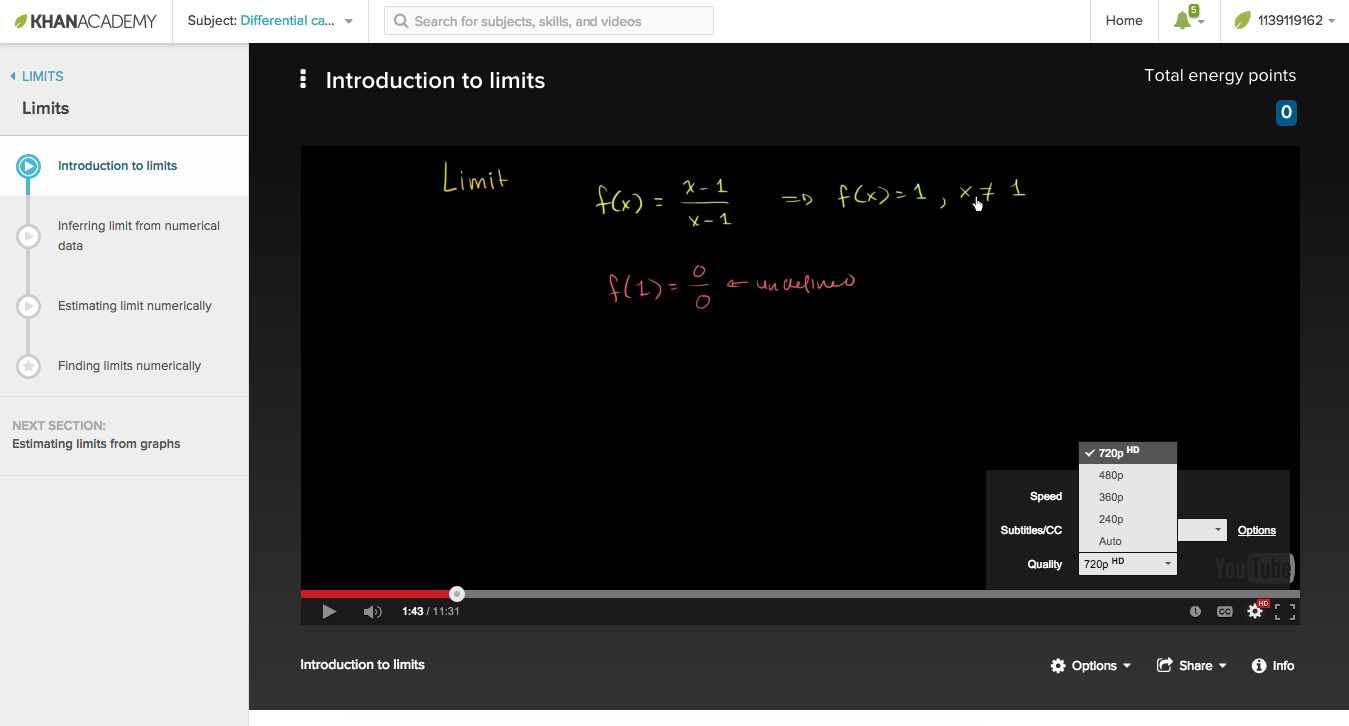
\includegraphics[width=30mm,natwidth=1348px,natheight=726px]{../img/khan-academy-screenshot.png}
	\caption{Khan Academy lesson}
	\label{fig:khan-screen}
\end{figure}
\chapter{The Vector Video project}

In the spring of 2014 the people behind ``Khanova Škola'' -- the Czech branch of the Khan Academy -- were looking for a person to develop an experimental video technology based on vector graphics. Their idea was to record raw data of user's input as he creates a Khan-style-video and later, when another user watches the video, draw the video scaled to match user's device's resolution and thus achieving maximum quality of the output. The result of this will be that the video will never become obsolete because it's quality isn not keeping up with the times.

Thanks to the sparse nature of vectors, in comparison to bitmaps, the data consumption might also be reduced or at least similar. This animation would also be linked to an audio track of authors voice commentary forming a complex KSV video suitable for educational purposes.

\section{Video recording tool requirements}
User, who wants to create a new video, should enter a website in his web browser and without installing any additional software start recording a video using his mouse, touchscreen or digital stylus and a microphone. This video should then be uploaded to the server.

If the user uses a pressure-sensitive stylus, then the applied pressure during drawing should be recorded too. The more pressure the user applies, the thicker the line will be and vice versa. Using this specific hardware might require additional drivers or specific software installed.

Different brush sizes, brush colors and background colors are available for the user. User should be able to erase certain parts of the canvas or the whole canvas at once. User should be able to pause and continue recording at any time.

Lines are immediately rendered on the screen as the user draws them, so he sees exactly the same output as the viewer will when he is playing the video later. All the raw data collected from the user should be stored, including the data that have no effect for video playback, like recording cursor movement while recording is paused. This will allow the user to simulate the process of video recording in the future and use it for further post-processing in any distant future. Recording of this redundant information should be optional.

\section{Video player requirements}
Any user should be able to play vector video on-line in all major modern web browsers without any special software or plugin installed, including mobile browsers.

Video should be scaled appropriately to the size of the player and device's screen resolution. The lines should have the same shape as the author has intended.

User can pause and continue with the playback of the video at any time. User can skip to any point of the video either forward or backward.

If the author of the video had recorded his voice, it must be played along the video. Audio must be synchronized with the video whenever user plays or pauses the video or when he skips to a different point on the time line.

User interface should be intuitive and easy to use either on a desktop computer using mouse and keyboard, but also with touchscreens on mobile devices.

\section{Goal of this thesis}

The result of this thesis should be an open-source library suitable for extending any web application with the abilities of recording and playing Khan Academy style videos in modern web browsers. An appropriate vector-based format should be chosen or defined to store video data.

The library should be easily adjustable and configurable for different purposes. User interface should be fully translatable to any language.
\chapter{Analysis}

\subsection{Technical requirements}
The overall project consists of two separate tools --- the recorder and the player. Each of these tools behaves differently and will be used by different people. While the video player will be used by general audience, the recorder will be used by a much narrower group of content creators.

The recording tool will capture the movement of a virtual chalk and lines drawn on a virtual blackboard, as well as voice of the author using a microphone. The recorder data will be then sent to the server, where it should be stored. The video player will receive previousely recorded data and display the movement of the chalk and lines created by the author while playing the voice comment. It is required that the video player will placed in a web page and it must run well in a all modern web browsers without requiring installation of any non-standard plugins or codecs and thus making it easy for a potential viewer to watch contents of the video.

For the purposes of recording, the tool must be able to capture the input from a microphone, track mouse movement and left mouse button state, collect information from Wacom graphics tablet devices and draw lines on screen. What the creator sees should be the same as what the end user will watch later.

\subsection{Available techonologies}
Web is a huge and fast growing environment. In only a few years, it has become a universal place for exchanging and presenting information. This put the web in the focus of many software companies and organizations and as a result, many different technologies for developing rich interactive applications (RIA) have been created. Some of them have already faded into obscurity, other are just emerging. One of the main limitations in the selection of the right technology for developing web application is their compatibility with operating systems and web browsers.

\subsubsection{Java applets}
Java applets are used for creating interactive applications withing web browser. Java applets meet all the specified technical requirements of both video player and recording tool.

Java applets are written in any language, that can be compiled into bytecode, this bytecode is then downloaded to the web browser and then run using Java Virtual Machine (JVM). This means that to be able to run a Java applet, user needs to have JVM installed on the device and an installed and allowed Java plugin in user's browser. This isn't a problem for desktop systems as Java is open source, but there is no support for mobile operating systems such as iOS and Android \cite{}. 

\subsubsection{Adobe Flash}
Adobe Flash is a multimedia and software platform used for creating vector graphics, animations and games. Flash has all required features: vector graphics manipulation, working with XML, mouse input capturing, microphone input, and audio streaming \cite{}. 

To view Flash animations or to execute Flash applications, Adobe Flash Player is needed. Adobe Flash Player is available and being developed for all major operating systems, although that is not true for mobile platforms. There was never any support for Apple iOS \cite{} and in 2012 deveolpment of Flash for Android was discontinued \cite{}. Using Adobe Flash would mean to exclude most users of tablets and smartphones \cite{}, which is a large disadvantage of this technology.

\subsubsection{Microsoft Silverlight}
Microsoft Silverlight \cite{} a development tool for creating web applications. It is based on the .NET Framework and it is similar to Java applets and Adobe Flash. It was Microsoft's attempt to compete Adobe Flash, but wasn't well adopted.

Silverlight comes as a plugin for web browsers. It is free, altough the list of supported browsers is even smaller \cite{} than the one of Adobe Flash consisting of exclusively desktop operating systems. Development of Silverlight was also discontinued by Microsoft in 2012 and the combination of these facts makes it unsuitable for this project.

\subsubsection{HTML5}
HTML5 is the fifth revision of Hypertext Markup Language (HTML) standard of World Wide Web Consortium (W3C). It has been given the Recommendation status in the end of 2014 and all crutial aspects of both tools can be implemented using the proposed standard. Tracking mouse was long supported even in older specifications of HTML and ECMA Script (familiarly known rather as Java Script). Wacom provides a plugin and ``Wacom WebPlugin Feel™ Multi-Touch API'' [http://www.wacomeng.com/web/WebPluginTouchAPI.htm] for web browsers providing access to precise data from graphical tablets from this manufacturer. Vector graphics are supported through the Scalable Vector Graphics (SVG) format \cite{} and it can be manipulated through Document Object Model (DOM) API \cite{}, as well as any other XML content. MediaStream API \cite{} enables access to audio input from user's microphone. The ``<audio>'' tag can be used to stream audio files and play them in the web browser.

While HTML5 is a new technology, many of the most important features have already been implemented in some web browsers, like Google Chrome and Mozilla Firefox. More specifically all the features needed to implement video player are supported in the latest versions of all major web browsers. The only catch might be a disagreement on supported audio file formats among the developers of web browsers. This can be overcome by converting the audio into the most widely used formats and providing them to the browser, which will then choose the one it supports.

The features needed by the recording tool, like the MediaStream API, are more specific and the number of browsers supporting these features is smaller, but this won't be an issue for content creators, who can easily install a supported web browser on all desktop platforms and even some mobile ones. Also a fast development in this area is expected and these features will be most likely implemented in all major browsers soon.

\subsection{Conclusion}
The bottleneck of most of the technologies is their support in mobile devices. These devices don't allow some of the above mentioned technologies to run inside them. As the popularity and market share of mobile devices grows, supporting them is a high priority. This eventually leads to only one option, and that is HTML5. All major web browsers have the features needed to create the video player, including the versions of browsers for mobile devices.

\subsection{Possible issues and known limitations}
Web browsers are developed by several companies and 



Mobile OS browsers limitations - audio recording.

Audio recording - large ammount of data - uncompressed - which approach of upload to choose? The most simple - create wav in browser and upload it via multipart form. The more complicated approach - continuous stream using WebSockets or WebRTC - need of specific web server process implementation.

\chapter{Vector Screencast file format}
\label{c:the-format}

SVG format is common and is implemented in web browsers and in many programs. These programs can open an SVG image and draw its contents. The idea is to create an SVG file, which contains all the information needed using custom namespace attributes and elements and shows the state of the blackboard at the end of recording.

A valid SVG document must have an \textit{svg} root element with specific namespace attributes and specified \textit{width} and \textit{height} attributes. For the purpose of extending the document, a new namespace \textit{http://www.rozsival.com/2015/vector-screencast} is added with the prefix \textit{``a''}. An example of an empty SVG document with this namespace looks as follows:

\begin{lstlisting}
<?xml version="1.0"?>
<svg version="1.1"
        width="470"
        height="100"
        xmlns="http://www.w3.org/2000/svg"
        xmlns:a="http://www.rozsival.com/2015/vector-screencast">

</svg>
\end{lstlisting}

SVG specification allows inclusion of elements and attributes from foreign namespaces anywhere with the SVG context. Attributes from foreign namespaces might be attached to any element. Both elements and attributes will be included in the DOM by the SVG user agent, but will be ignored otherwise \cite{svg_exteding}.

Vector Screencast \verb|<svg>| root element must have two child elements: \verb|<metadata />| and \verb|<g a:type="chunks" />|

SVG \verb|<g>| element is intended for grouping related graphics elements. These groups might be also nested.

\section{Video Metadata}
The first child element of the \verb|<svg>| element must be a \verb|<metadata>| element. This element must contain these child elements:

\paragraph{\texttt{\textless a:width\textgreater} and \texttt{\textless a:height\textgreater}}
The content is the original width and height of the blackboard. These numbers will be used to correct coordinates when playing the video with different resolution. The \verb|width| and \verb|height| attributes of the \verb|<svg>| element may contain different values.

\paragraph{\texttt{\textless a:length\textgreater}}
The content is the duration of the video in milliseconds.

\paragraph{\texttt{\textless a:audio\textgreater}}
Contains the list of audio sources as child elements.

\subparagraph{\texttt{\textless a:source\textgreater}}
Defines one audio source. It has two attributes: \verb|a:src| -- containing the URL of the audio source, and \verb|a:type| -- containing the MIME type of the audio source.

\section{Video Chunks}
Video is divided into smaller consequent parts, called \textit{chunks}. Chunks have variable time duration based on user's behaviour. These chunks are logical units of the video, each of them can be rendered at once as one graphics primitive. This helps optimize skipping parts of the video. Some chunks can be skipped entirely as the canvas will be cleared at some point after the very chunk is rendered, but before the target time point is reached.

There are three types of chunks: \textit{path}, \textit{erase}, and \textit{void} cuhnk. Each chunk is stored as one SVG group element with a specific \verb|a:type| attribute (\textit{path}, \textit{erase}, \textit{void}) and an \verb|a:t| attribute, which is the time, when this chunk starts to be processed, in milliseconds. Chunks contain the prerendered graphics primitive and a list of animation commands.

\paragraph{``Path''}
This type of chunk represents one line the user draws. The first child element is an SVG \verb|<path>| element. The \verb|fill| attribute should correspond to the real color of the path, but is not neccessary for later screencast playing. The data attribute \verb|d| includes serialized information about the segments of the path in the form of valid SVG path instructions. For more details about the serialization and deserialization of this data, see section~\ref{sec:path_serialization} on page~\pageref{sec:path_serialization}. One or more child elements might follow after the \verb|<path>|, all of which must be animation command elements.

\paragraph{``Erase''}
This type of chunk represents clearing the whole canvas with one color. The first child element is an SVG \verb|<rect>| element. The \verb|fill| attribute should correspond to the real color of the new background. One or more child elements might follow after the \verb|<rect>|, all of which must be animation command elements.

\paragraph{``Void''}
This type of chunk does not render anything on the canvas. It might contain one or more child elements, all of which must be animation command elements.

\section{Animation Commands}
Animation commands are necessary for correct actions' timing during the video. Chunks contain the information of how the resulting primitive looks like, commands contain user's gradual forming of these primitives.

Animation command must be a child element of a chunk element. Every command has an \verb|a:t| attribute with a timestamp of the action in milliseconds. Time value is relative to the time value of its parent chunk -- this decreases the number of digits of each time value and thus the number of bytes needed for textual representation of the value. The value of the time attribute of an element must be greater or equal to the values of preceding sibling action elements. If command does not have this attribute, it is assumed that it has zero value -- this decreases the size of commands created while the recording is paused.

\paragraph{\texttt{\textless a:m\textgreater}}
\textit{Move cursor} command tells the player to move cursor to a specific position defined by attributes \verb|a:x| and \verb|a:y|.

\paragraph{\texttt{\textless a:c\textgreater}}
\textit{Change color} command tells the player to switch current brush color according to the value of \verb|a:c| attribute. Value of the attribute must be a valid CSS color value\footnote{http://www.w3.org/TR/CSS2/syndata.html\#value-def-color}.

\paragraph{\texttt{\textless a:s\textgreater}}
\textit{Change brush size} command tells the player to change current brush size to the value of \verb|a:w| attribute. The units of this value are pixels and the size must be corrected according to the width and height stated in \textit{metadata}.

\paragraph{\texttt{\textless a:d\textgreater}}
\textit{Draw next segment} will render the next segment of the current path with current brush color and size. This command doesn't carry any additional information, all the information about the segment is carried by the \textit{path} chunk. \textit{Draw next segment} commands can be present only in a \textit{path} chunk. There must not be any \textit{change color} or \textit{change brush size} command between the first \textit{draw next segment} command and the last one inside one \textit{path} chunk -- color or size cannot be changed in the middle of a line.
\chapter{Implementation}
How the source was designed and maintained. Mention that the development of the code can be found on Github?

\section{HTML5}
What is HTML5, what parts are needed. Compatibility of these technologies in browsers. A chart of people using a compatible browser? Playing should be possible in the vast majority of browsers today and the prognose is good.





\subsection{Event driven programming}
When creating the architecture of Vector Screencast, a lot of 

The Event Aggregator mechanism is imlemented through the ``VideoEvents'' object literal. This object provides a very simple interface for registering and triggering callbacks for specific events.














\subsection{Working with XML data}
Using jQuery here.


\subsection{Drawing lines}
At the time of recording, mouse coordinates relative to the drawing board are captured along with the pressure of the pen on a drawing board or the state of the left mouse button. This data is then used to draw a line with a changing width at the moment of recording as a visual feedback for the person recording and then every time the video will be replayed. The outcome of the rendering phase should be the same every time so the intention of the creator is perserved. On the other hand, the rendering algorithm might be improved in the future and the video could be rendered using to this algorithm without any editing.

Rendering at the time of playback gives us the opportunity to adjust the outcome to the environment of the end user. This means that the result can be sharp on every display resolution.


\subsection{Audio capturing}

\subsection{Audio processing}








\subsection{Input handling}
Detecting mouse and keyboard input is easy, there is a plugin for Wacom darwing tablets and it is supported in Vector Screencast - different pressure means different thickness.
\chapter{Integration into other applications}
How to integrate the player and the recorder into another web application.

\section{Video player}
The frontend. And a short comment on how to deal with large data transfers - CDN like Amazon S3, Google App Platform, Microsoft Azure...

\section{Video recording}
The frontend. And the server program. A short comment on how to implement the the website backend - insert the data into a database.
\chapter{Users' documentation}
The Video Screencast tools were designed to be easy to use and allow users to work with them right away. The following sections summarize the way user can interact with the default UI of both library tools. UI might be changed by the user of the library and the user experience might change. It is then up to the user of the library to explain the specifics of the new interface to the screencast authors and audience.

\section{Vector Screencast Player}
Once the screencast is ready to be played, you can start learning. You should see a simillar interface to the one shown at figure~\ref{fig:player}. The area of the player consists of two main parts -- the blackboard and control bar.

\begin{figure}
	\centering
		\includegraphics[width=150mm]{../img/player_screenshot.eps}
		\caption{The default UI of Vector Screencast Player\label{fig:player}}
\end{figure}

\paragraph{Play/Pause/Replay}
In the bottom left part of the screencast player UI there is a button with a ``play'' icon. You start or resume the playback by clicking on the button.

When the screencast is playing, the icon changes to a ``pause'' icon. By clicking on the same button, playback of the screencast is paused. The icon will then change to the ``play'' icon.

When the end is reached, the playback stops and the icon changes to a ``replay'' icon. When you click on the button now, playback will start over from the very beginning.

Instead of clicking on the button, you may press the spacebar key on your keyboard, if you have one. You can also click or tap the blackboard to play/pause playback.

\paragraph{Skipping parts of the screencast}
In the top section of the control bar there is a timeline. It shows progress of the video. You can click on the timeline to change current position of the video to the one corresponding to your selection. If you hover your mouse over the timeline, a box with time information of that point will appear. On touch some devices, you might have to tap second time to confirm the selected position.

Instead of clicking on the timeline, you can press left and right arrow keys on your keyboard. Each stroke of the keys will skip five seconds of the screencast forwards or backwards.

\paragraph{Control bar hiding}
When the screencast is playing, the control bar is not needed and could be hidden. To turn hiding on and off, press the right most button in the control bar. You probably would not see the effect immediatelly. The control bar hides only if the video is being played. It is shown automatically when the video is paused or reaches end. It is shown also whenever you hover your mouse over the remaining visible parts of the control bar.

\paragraph{Audio controls}
You can control audio volume by clicking on buttons in the ``Volume controls'' section of the control bar. Volume can be decreased, increased or muted/unmuted.


\section{Vector Screencast Recorder}
After you enter the page with the recorder, you should see a simillar interface to the one shown at figure~\ref{fig:recorder}. The area of the recording tool consists of two main parts -- the blackboard and control bar.

\begin{figure}
	\centering
		\includegraphics[width=150mm]{../img/recorder_screenshot.eps}		
		\caption{The default UI of Vector Screencast Recorder\label{fig:recorder}}
\end{figure}

\paragraph{Microphone access and audio recording}
Your browser will ask you to allow access to your microphone. Confirming this prompt is neccessary for audio recording. If this message does not show, your computer probably does not have a microphone, your browser does not support audio recording or you have denied access to your microphone earlier. 

A white not crossed out icon of a microphone should appear in the ``Audio recording'' section of the control panel. If the icon is red, audio recording is not available. Please make sure you use the latest version of your web browser and check you browser and operating system microphone settings if you encounter problems.

If you do not want to record audio or you want to mute the microphone in the middle of recording, press the microphone button. You will resume recording your voice by clicking the button one more time.

\paragraph{Drawing}
You can start drawing as soon as audio recording is set up. You can now prepare the inital look of the screen. When you click the ``Start'' button, your cursor movement and voice will start being recorded. You can pause and resume recording at any time and as many times as you want.

Before you start drawing a line, select brush size and brush color from the palette in the control bar. Draw a line by pressing your mouse, stylus or touching your touchscreen and moving the cursor around the blackboard. End a line by releasing mouse button, stylus pressure of lifting your finger.

It is recommended to use a pressure-sensitive graphics tablet to achieve best results. If you use a touchscreen, consider using a specialized stylus instead of fingers to create better drawings.

\paragraph{Erasing}
If you want to clear the whole blackboard, select a color from the color palette and click on the button in the ``Erase everything'' section of the control bar. The color of the button should correspond to your previousely selected color. Everything will be removed from the balckboard and the background color of the ``\textit{black}board'' will be set to the selected color.

\paragraph{Saving the recording}
After you have finished recording and the recording is stopped, press the ``Upload'' button. The data will be uploaded to the server. This process will take some time, even a few minutes, depending on your Internet connection uplink speed and the length of your recording. After the video is uploaded, you will be informed




\chapter*{Conclusion}
\addcontentsline{toc}{chapter}{Conclusion}

The goal of this thesis was to create an open-source library, which will allow users to create educational websites for creating and playing KSVs. The library uses a vector-based approach. Video is rendered with respect to user's screen resolution and the size of the viewport.

The project of Vector Screencast is available online as a public Git repository\footnote{https://github.com/simonrozsival/vectorvideo}. The library is written in a programming language, which should be easy to learn for all web developers. The library uses an object oriented design and is very modular, which makes it easy to extend with a custom rendering method, file format support or user interface.

\paragraph{File format} Vector Screencast data is stored in a specificaly formed SVG document extended with a foreign namespace. The data contains information of author's cursor movement and applied pressure and prerendered lines. This type of animation cannot be viewed in any other video player, but a preview of the final state of the blackboard is displayed when the file is opened in a regular SVG viewer. Audio is recorded as an uncompressed WAV file. This file should be converted into one or more common binary audio formats, with respect to web browsers support of audio formats. 

\subparagraph{File size}
@todo

\section{Future work}
The library is ready and anyone can use it today in his website for creating and playing KSVs. There are tools for drawing lines of different widths and colors onto a virtual canvas, erasing parts of the canvas and clearing the whole canvas. Some authors might be missing some tools they use in their bitmap editors when recording KSV -- including bitmap images or photos, using a text tool or drawing straight lines. It would not be hard to implement these tools, but it would have to be thought over, whether they do not breach the idea of simple, natural look of KSV.

\paragraph{Binary file format}
SVG has proven to be a sufficient container for Vector Screencast data. A binary format should be used to achieve more data savings. Most of the data consists of coordinates and time values. Numbers are stored as strings in XML. Each digit character in an UTF-8 document takes up 1~B of data storage. Each component of a coordinate is a number with typical value in the range of 0 to 9999 with several decimal places -- the library allows three decimal places at maximum. A typical coordinate component value, like ``123.5'', takes up more than 4~B, with the decimal dot character included. If these numbers were saved binary as a 32-bit integer, or 32-bit floating point number, it would take up only 4 bytes of memory in total while maintaining the same precission in most cases.

This project was designed to be independent on a specific file format. The library can be easily extended to support different file structures without editing its source code.

\paragraph{Library for native mobile applications}
The library can be used in any HTML website and playback of a screencast will work well in all modern mobile web browsers. However, users of tablets and smartphones are used to obtaining application in application markets and use them instead of web browsers. Many developers would certainely welcome a Vector Screencast comonent, they could use in their native Android or iOS app. 


\subsection*{Known issues}
\paragraph{Audio recording} \textit{ScriptProcessorNode} interface is deprecated in W3C Editor's Draft of \textit{Web Audio API} from 21 June 2015 \cite{mic_deprecated}. This interface is used in this project and should be replaced using \textit{Audio Workers}, when the specification is finalized \cite{audio_worker}. 

\paragraph{Demo audio server} \textit{Audio recording server} program, which is included in the project as a demo, should be rewritten. This tool is not very robust and sometimes fails to save the data, it receives through a WebSocket, to a file on the server. Users must write this server program themselves at the moment.

%%% Seznam použité literatury
%%% Seznam použité literatury je zpracován podle platných standardů. Povinnou citační
%%% normou pro bakalářskou práci je ISO 690. Jména časopisů lze uvádět zkráceně, ale jen
%%% v kodifikované podobě. Všechny použité zdroje a prameny musí být řádně citovány.

\def\bibname{Bibliography}
\begin{thebibliography}{99}
\addcontentsline{toc}{chapter}{\bibname}

%\bibitem{lamport94}
%  {\sc Lamport,} Leslie.
%  \emph{\LaTeX: A Document Preparation System}.
%  2. vydání.
%  Massachusetts: Addison Wesley, 1994.
%  ISBN 0-201-52983-1.

\bibitem{1}
{\sc Bower,} Beverly L. {\sc Hardy,} Kimberly P.
\emph{From correspondence to cyberspace: Changes and challenges in distance education} [online].
New Directions for Community Colleges, Volume 2004, Issue 128, pages 5–12.
\bibitem{2}
John Oliver: Student Debt, HBO [online] 9/7/2015, available at https://www.youtube.com/watch?v=P8pjd1QEA0c
\bibitem{3}
Bill Gates: Online, All Students Sit in the Front Row [online], posted on November 18, 2014, seen on 3/12/2015, available at http://www.gatesnotes.com/Education/Colleges-Without-Walls-Arizona
\bibitem{4}
Jessica Leber: In the Developing World, MOOCs Start to Get Real [online], MIT Technology Review, published on March 15, 2013, available at http://www.technologyreview.com/news/512256/in-the-developing-world-moocs-start-to-get-real/
\bibitem{5}
Kepler [online], http://kepler.org/
\bibitem{6}
Generation Rwanda [online], http://www.generationrwanda.org/
\bibitem{7}
Moodle, https://moodle.org
\bibitem{8}
Moodle statistics, https://moodle.net/stats/
\bibitem{9}
Coursera [online], 3/13/2015, available at https://www.coursera.org/about/
\bibitem{10}
Youtube.com, https://www.youtube.com
\bibitem{11}
Alexa Internet, http://www.alexa.com/topsites
\bibitem{12}
Numberphile Youtube channel, https://www.youtube.com/user/numberphile
\bibitem{13}
Veritasium Youtube channel, https://www.youtube.com/user/veritasium
\bibitem{14}
Khan Academy Youtube channel, https://www.youtube.com/user/khanacademy
\bibitem{15}
Khanova škola, https://khanovaskola.cz


% 05_Choice of technologies

\bibitem{}
Oracle, Java.com, How do I get Java for Mobile device? [online] viewed April 16, 2015
http://www.java.com/en/download/faq/java_mobile.xml


\bibitem{}
%%% FLASH DOCUMENTATION OR FEATURES?? %%%

\bibitem{}
Steve Jobs, Apple.com, Thoughts on Flash, published April 2010, viewed April 16, 2015 [online]
http://www.apple.com/hotnews/thoughts-on-flash

\bibitem{}
Adobe Blog, An Update on Flash Player and Android, published June 28, 2012, viewed April 16, 2015 [online]
http://blogs.adobe.com/flashplayer/2012/06/flash-player-and-android-update.html

\bibitem{}
Bosomworth Danyl, SmartInsights.com, Mobile Marketing Statistics 2015, published January 15, 2015, viewed April 16, 2015 [online]
http://www.smartinsights.com/mobile-marketing/mobile-marketing-analytics/mobile-marketing-statistics/

\bibitem{}
Microsoft Silverlight, http://www.microsoft.com/silverlight/

\bibitem{}
Microsoft Silverlight, Get Microsoft Silverlight, viewed April 16, 2015 [online]

\end{thebibliography}


%%% Použité zkratky v bakalářské práci, existují-li, včetně jejich vysvětlení.
\chapwithtoc{List of Abbreviations}
\printnomenclature



%%% Přílohy k bakalářské práci, existují-li (různé dodatky jako výpisy programů,
%%% diagramy apod.). Každá příloha musí být alespoň jednou odkazována z vlastního
%%% textu práce. Přílohy se číslují.
%\chapwithtoc{Attachments}

\openright
\end{document}